\documentclass[a4paper,12pt]{report}

\usepackage{alltt, fancyvrb, url}
\usepackage{graphicx}
\usepackage[utf8]{inputenc}
\usepackage{float}
\usepackage{hyperref}
\usepackage{caption}
\usepackage[caption = false]{subfig}

\usepackage[italian]{babel}

\usepackage[italian]{cleveref}

\title{TaflGames\\\large Relazione per il progetto \\ del corso di \\ Object-Oriented Programming \\ A.A. 2022/23}
\author{Alin Stefan Bordeianu \\ Elena Boschetti \\ Andrea Piermattei \\ Margherita Raponi}
\date{\today}	

\begin{document}

\maketitle

\tableofcontents

\chapter{Analisi}

Lo scopo del progetto è la realizzazione di un'applicazione incentrata su un gioco da tavolo denominato “Hnefatafl”, appartenente alla famiglia dei Tafl Games, un insieme di giochi di origine nordica e celtica. 

\section{Requisiti}

\subsubsection{Requisiti funzionali}

\begin{itemize}
	\item Sono previste \textbf{due modalità di gioco}: una corrisponde alla versione originale, mentre l'altra è una variante di nostra invenzione che presenta degli elementi aggiuntivi.
	\item Entrambe le modalità di gioco si svolgono su una griglia quadrata di dimensione 11x11 e prevedono due giocatori, i quali dispongono di una squadra di pedine ciascuno. Un giocatore ha il ruolo di \textbf{difensore} e il suo compito è proteggere il re, che fa parte della sua squadra, fino a portarlo ad una delle uscite che si trovano agli angoli della griglia. L'altro giocatore, invece, ha il ruolo di \textbf{attaccante} e il suo scopo è catturare il re circondandolo con le proprie pedine.
	\item Entrambe le modalità prevedono la presenza di \textbf{pedine classiche} e di un \textbf{re}. La squadra del difensore è composta da un re e da 12 pedine classiche, inizialmente posizionate nella parte centrale della griglia, mentre la squadra dell'attaccante è composta da 24 pedine classiche distribuite sui quattro bordi della griglia. Le pedine si possono muovere orizzontalmente o verticalmente e non è possibile oltrepassare o sovrapporre altre pedine. Una pedina classica viene mangiata quando vengono posizionate due pedine nemiche in due celle adiacenti ad essa e opposte (ad esempio, a sinistra e a destra della pedina). Il re, invece, viene mangiato quando è circondato su tutti e quattro le celle adiacenti da quattro pedine dell'attaccante; tale condizione stabilisce la vittoria dell'attaccante.
	\item Entrambe la modalità prevedono tre tipi di celle.
	\begin{itemize}
		\item Le \textbf{celle classiche} non hanno alcun effetto o comportamento distintivo.
		\item Il \textbf{trono} è la cella in cui è posizionato inizialmente il re. Ha la particolarità di avere una propria hitbox, comportandosi come una pedina se si cerca di fare una mangiata nelle celle adiacenti ad esso.
		\item Le \textbf{uscite} sono celle presenti ad ognuno dei quattro angoli della griglia; se una di esse è raggiunta dal re, allora il difensore vince. Chiaramente, non è possibile posizionare sulle uscite nessuna pedina che non sia il re.
	\end{itemize}
	\item La variante del gioco prevede quattro ulteriori tipi di pedine e due ulteriori tipi di celle.
	\begin{itemize}
		\item Gli \textbf{slider} sono delle celle speciali che causano lo spostamento di una pedina alla cella più lontana possibile nella direzione indicata dalla freccia sulla cella.
		\item Le \textbf{tombe} vengono posizionate in corrispondenza delle celle in cui viene mangiata una pedina.
		\item La \textbf{regina} è una pedina speciale che ha il potere di riportare in gioco una pedina alleata, posizionandosi in una cella adiacente ad una tomba in corrispondenza della quale è stata mangiata tale pedina.
		\item L'\textbf{arciere} ha l'abilità di partecipare ad una mangiata anche a distanza, minacciando le pedine che si trovano ad una distanza massima di tre celle sulla stessa riga o colonna in cui l'arciere viene posizionato.
		\item Lo \textbf{scudo} ha il potere di sopravvivere al primo tentativo di mangiata che subisce.
		\item Lo \textbf{swapper} può scambiare la propria posizione con una pedina avversaria, escluso il re.
	Sia all'attaccante che al difensore sono assegnati una regina, due arcieri, due scudi e uno swapper, Al difensore è assegnato un re come nella modalità classica. Tutte le altre pedine rimanenti (18 per l'attaccante e 6 per il difensore) sono pedine classiche.
	\end{itemize}
	\item Al momento della scelta della modalità di gioco, deve essere possibile visualizzare il regolamento di entrambe le modalità.
	\item Durante il suo turno, ogni giocatore deve avere la possibilità di annullare la propria mossa ed effettuarne un'altra prima di passare il turno all'altro giocatore.
	\item Al termine della partita, i giocatori devono avere la possibilità registrare il proprio risultato, immettendo anche il proprio nome; i risultati registrati dovranno poter essere visualizzati su una leaderboard.
\end{itemize}

\subsubsection{Requisiti non funzionali}

\begin{itemize}
	\item L'applicazione deve essere in grado di gestire correttamente le risorse legate alla configurazione di gioco, alla parte grafica e al salvataggio e caricamento della leaderboard.
	\item Deve essere garantita all'utente un'interazione fluida con l'applicazione.
\end{itemize}

\section{Analisi e modello del dominio}

Il modello del dominio dell'applicazione corrisponde al concetto di partita, la quale incapsula tutto ciò che concerne la logica del gioco. L'entità centrale nel contesto della partita è la griglia di gioco (\texttt{Board}), che si occupa delle interazioni fra tutti gli altri elmenti del dominio (\texttt{Piece} e \texttt{Cell}).

La partita (rappresentata dal \texttt{Model}) si occupa della gestione dei turni di gioco e comunica con la \texttt{Board} per il controllo della validità delle mosse e il loro compimento e per ottenere il risultato della partita qualora vi siano le condizioni per la sua fine.

Internamente, la \texttt{Board} contiene la collezione di celle e la collezione di pedine. Ogni cella è modellata dall'interfaccia \texttt{Cell} e ogni pedina è modellata dall'interfaccia \texttt{Piece}; tali interfacce definiscono il modo in cui la \texttt{Board} può interrogare e modificare lo stato delle pedine per applicare tutte le meccaniche di gioco, cioè spostamenti, mangiate ed effetti speciali.

\begin{figure}[H]
\centering
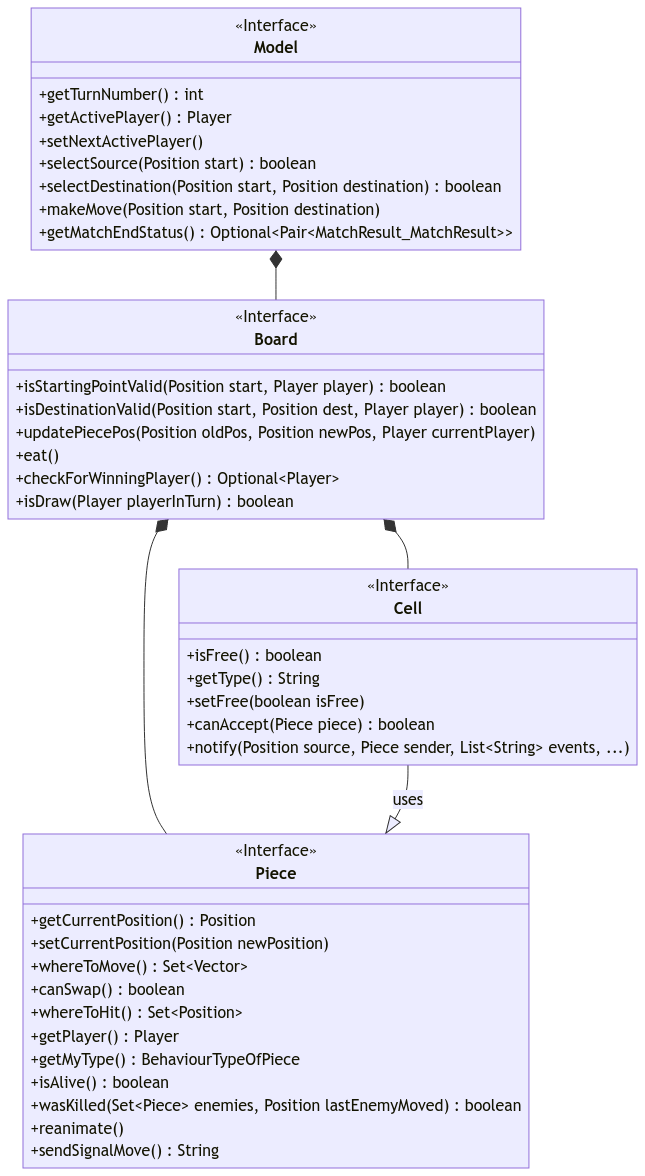
\includegraphics[width=0.8\textwidth]{images/analysis.png}
\caption{Schema UML del modello del dominio.}
\label{images:analysis}
\end{figure}

\chapter{Design}

\section{Architettura}

Come pattern architetturale, è stato scelto MVC in quanto permette di separare la logica dell'applicazione da ciò che viene mostrato all'utente, portando ad un'organizzazione interna dell'applicazione più pulita e più facilmente gestibile.

L'interfaccia \texttt{Model} racchiude la logica del dominio di gioco, isolandola da tutti gli altri componenti dell'architettura. Idealmente, il gioco potrebbe funzionare anche senza alcuna componente grafica, direttamente ricevendo input da linea di comando.

Il \texttt{Controller} si occupa del coordinamento fra Model e View, permettendo ai cambiamenti di stato della partita di essere visualizzati dall'utente. Il Controller gestisce anche alcune risorse non inerenti alla parte grafica dell'applicazione, ad esempio file di configurazione per il setup della partita e file per il salvataggio e il caricamento della leaderboard.

La \texttt{View} si occupa del rendering grafico delle varie schermate dell'applicazione. A ciascuna schermata è associata una specifica \texttt{Scene} e ciascuna di esse è legata ad un proprio \texttt{SceneController} che gestisce il comportamento della scena e la comunicazione tra la \texttt{Scene} stessa, la \texttt{View} (la quale è, in pratica, un container di \texttt{Scene}) e il \texttt{Controller}.

\section{Design dettagliato}

\subsection{Alin Stefan Bordeianu}

\subsection{Elena Boschetti}

\subsubsection{Match setup}

La fase di setup della partita prevede la creazione della griglia di gioco e la disposizione delle pedine su di essa; in termini di codice, ciò corrisponde alla creazione di un oggetto di tipo \texttt{Board} e all'inizializzazione delle collezioni di celle e pedine che essa conserva internamente. 

La costruzione delle due collezioni fa uso di due diversi builder: \\ \texttt{CellsCollectionBuilder} per la collezione di celle e \texttt{PiecesCollectionBuilder} per la collezione di pedine. Ogni metodo delle interfacce dei builder permette di aggiungere alle collezioni un sottoinsiemi di pedine e celle di un determinato tipo. Da notare che i builder ricevono le coordinate a cui posizionare celle e pedine dall'esterno (in quanto passate come parametri ai diversi metodi), quindi i builder operano in maniera indipendente dal modo in cui la configurazione iniziale di celle e pedine viene fornita.

La configurazione iniziale dipende dalla modalità di gioco (classica o variante). Il caricamento della configurazione per ogni modalità viene avviato mediante l'interfaccia \texttt{SettingsLoader}. Dietro tale interfaccia, si possono definire diverse possibilità per quanto riguarda il reperimento della configurazione, creando per ciascuna di esse una classe che implementi l'interfaccia. L'implementazione di \texttt{SettingsLoader} da me definita prevede il caricamento della configurazione da un file XML (uno per ogni modalità di gioco), ma sarebbe possibile definire altre classi che la ottengano in maniera differente. È una possibilità che potrebbe essere utile anche nel caso in cui si verifichino problemi: ad esempio, se il caricamento da file XML non va a buon fine per qualche motivo, si può decidere di procedere per una via alternativa, creando un nuovo tipo di loader che cerchi di reperire la configurazione in altro modo.

Per costruire le collezioni di pedine e celle secondo la configurazione, il \texttt{SettingsLoader} riceve un \texttt{CellsCollectionBuilder} e un \\ \texttt{PiecesCollectionBuilder} e interagisce con essi per creare e posizionare correttamente ogni tipologia di celle e pedine; ad esempio, il \texttt{SettingsLoader} ottiene le posizioni delle Exit Cells e successivamente chiama il metodo \texttt{addExits()} del \texttt{CellsCollectionBuilder}, passando tali posizioni. Una volta completata la costruzione delle due collezioni, esse vengono passate alla \texttt{Board} che viene istanziata, la quale viene a sua volta passata all'istanza di \texttt{Match} che viene creata.

\begin{figure}[H]
\centering
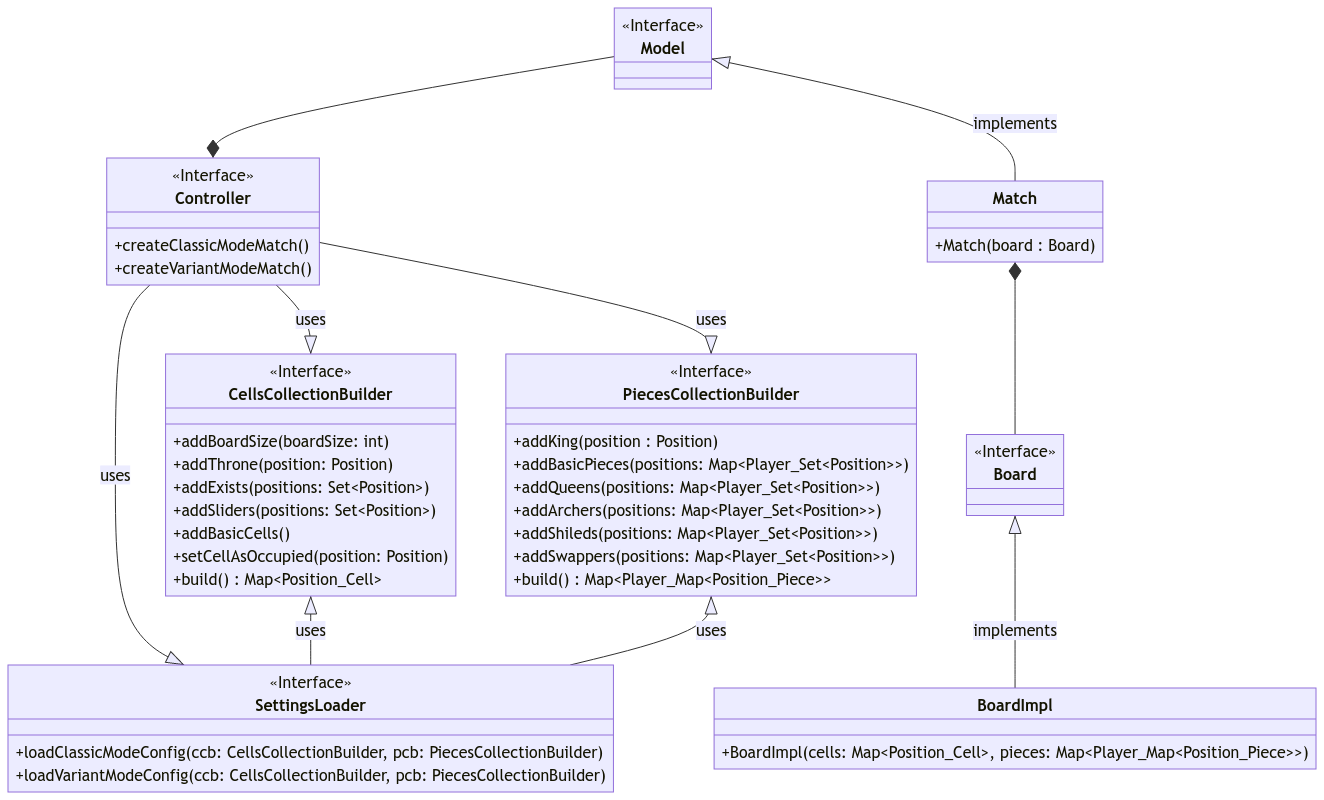
\includegraphics[width=\textwidth]{images/match-setup.png}
\caption{Schema UML che rappresenta l'interazione tra le entità coinvolte nel setup.}
\label{images:match-setup}
\end{figure}

\subsubsection{Scenes}

La view dell'applicazione, realizzata utilizzando la Java Swing API, è composta da un serie di scene.
L'implementazione della \texttt{View} prevede la creazione del container più esterno della view (un \texttt{JFrame}) e l'alternarsi delle diverse scene viene gestito impostando il frame con un opportuno layout (\texttt{CardLayout}) che consente di sostituire il container interno (un \texttt{JPanel}) che viene mostrato, il quale corrisponde alla scena.

Considerando la chiara differenza di ogni scena a livello grafico e le differenze di comportamento che ogni scena può avere (ad esempio, in risposta ad un input dell'utente), ho deciso di racchiudere il concetto di scena in un'entità a sè stante. L'interazione diretta con ogni scena avviene mediante l'interfaccia \texttt{Scene}, la quale consente di ottenere il container che costituisce la scena e di interagire con essa, ad esempio per il suo aggiornamento mediante il metodo \texttt{update()}. L'implementazione della \texttt{View} ha un riferimento alla \texttt{Scene} attualmente mostrata, il quale permette che un'interazione con la \texttt{View} abbia un effetto sulla scena corrente; ad esempio, se il controller dell'applicazione richiede l'aggiornamento della view mediante il metodo \texttt{update()} della \texttt{View}, in tale metodo viene richiamato il metodo \texttt{update()} della scena corrente.

Riflettendo sugli aspetti comuni che possono esserci tra le scene (ad esempio, la creazione del container e alcune sue impostazioni, oppure l'uso di altri parametri comuni, come il font) ho ritenuto che fosse utile definire una classe astratta (\texttt{AbstractScene}) che implementasse tali aspetti comuni tra le scene. 

Le implementazioni concrete di ogni scena estendono \texttt{AbstractScene} e definiscono tutto ciò che è inerente alla specifica scena; in particolare, ogni classe costruisce la parte grafica della scena e definisce altri eventuali metodi utili all'interazione dalla \texttt{View} alla scena. Ad esempio, qualora una scena debba avere un aggiornamento a seguito di un input dell'utente, esso può essere innescato chiamando il metodo \texttt{update()}, come detto precedentemente.

\begin{figure}[H]
\centering
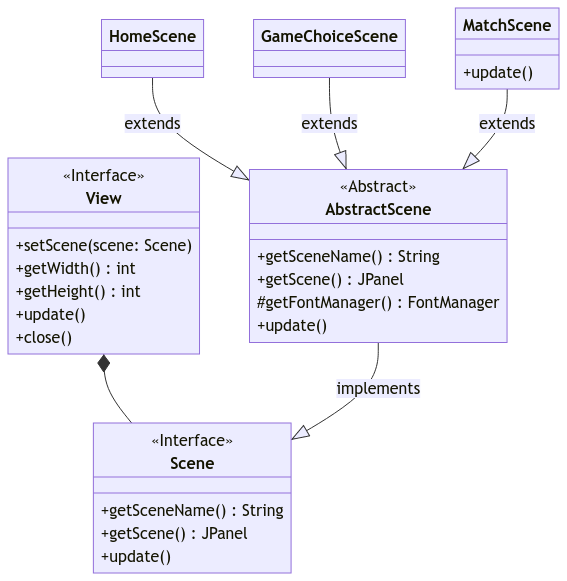
\includegraphics[width=0.75\textwidth]{images/scenes.png}
\caption{Schema UML che rappresenta il rapporto tra le entità che descrivono le scene della view. Sono mostrate solo le classi concrete che definiscono la schermata iniziale dell'applicazione (\texttt{HomeScene}), la schermata della scelta della modalità di gioco (\texttt{GameChoiceScene}) e la schermata della partita (\texttt{MatchScene}) a titolo esemplificativo.}
\label{images:scenes}
\end{figure}

In seguito a questa fase di design, mi sono occupata di implementare la scena della home del gioco (\texttt{HomeScene}), la scena della scelta della modalità di gioco (\texttt{GameChoiceScene}) e della scena che mostra il regolamento (\texttt{RulesScene}).

\subsubsection{Scene Controllers}

Nello sviluppo delle funzionalità delle scene, si è rivelato quasi sempre necessario che la scena interagisse con la \texttt{View} (che, come detto precedentemente, ha la funzione di wrapper della scena) o con il Controller dell'applicazione. Per questo motivo, ho deciso di introdurre delle entità, a cui mi riferisco con il termine "scene controllers", che regolano il comportamento della scena e che hanno il ruolo di mediatore tra \texttt{Scene}, \texttt{View} e \texttt{Controller}.

Tutte le scene hanno alcune funzionalità e necessità in comune, come il passaggio alla scena successiva o precedente e la necessità di conoscere le dimensioni della view per dimensionare i componenti interni; per questo motivo, ho deciso di raggruppare queste in un'unica interfaccia (\texttt{BasicSceneController}). Successivamente, ho notato che gli scene controllers condividevano anche parte della loro implementazione: ad esempio, contengono tutti un riferimento alla \texttt{View} e al \texttt{Controller} e ottengono dalla view le informazioni utili per il dimensionamento nello stesso modo; ho quindi deciso di realizzare una classe astratta (\texttt{AbstractSceneController}) che implementasse tali aspetti comuni.

Ogni scena ha poi le proprie specifiche funzionalità; ciò rende necessario che lo scene controller di ogni scena fornisca degli ulteriori metodi per poterle attuare, oltre a quelli stabiliti nel \texttt{BasicSceneController}. Ad esempio, Lo scene controller della home scene permette anche il passaggio alla scena che mostra gli high scores e permette di comunicare alla \texttt{View} la richiesta di chiusura dell'applicazione. Lo scene controller della scena di scelta del gioco, invece, permette la creazione della partita nella modalità scelta e permette di passare alla scena che mostra il regolamento di gioco. Ho quindi deciso che, per ogni scena, il rispettivo scene controller dovesse avere una propria interfaccia, che estendesse \texttt{BasicSceneController} (si veda la \Cref{images:scene-controllers-interfaces} in relazione agli esempi appena fatti). 

\begin{figure}[H]
\centering
\subfloat{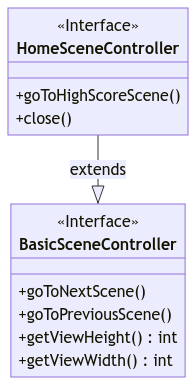
\includegraphics[width=0.3\textwidth]{images/home-scene-controller-interface.png}}
\subfloat{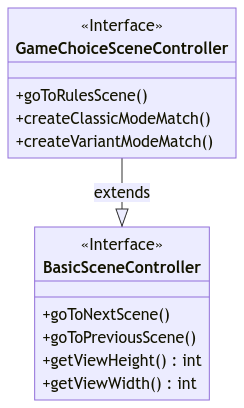
\includegraphics[width=0.3\textwidth]{images/game-choice-scene-controller-interface.png}}
\caption{Due esempi di interfaccia di due scene controllers.}
\label{images:scene-controllers-interfaces}
\end{figure}

L'implementazione di ogni scene controller deve quindi implementare la sua specifica interfaccia e estendere \texttt{AbstractSceneController}; di fatto, essa consiste solo nell'implementazione delle funzionalità specifiche della rispettiva scena.

\begin{figure}[H]
\centering
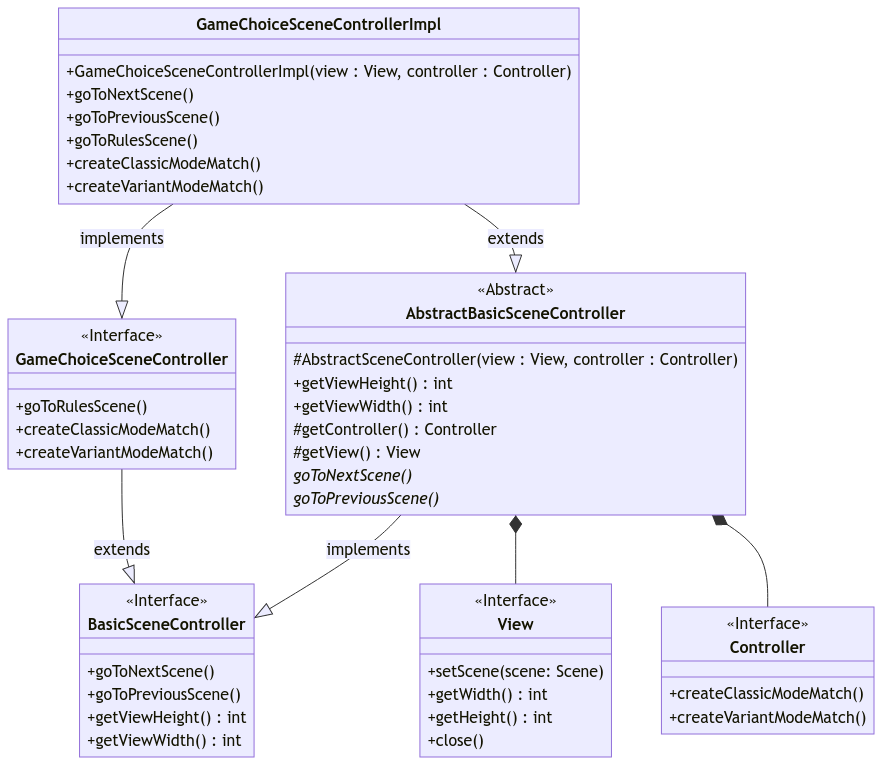
\includegraphics[width=\textwidth]{images/game-choice-scene-controller.png}
\caption{Schema UML che rappresenta il design di uno scene controller (in questo caso, lo scene controller della scena di scelta del gioco).}
\label{images:game-choice-scene-controller}
\end{figure}

In seguito a questa fase di design, mi sono occupata di implementare gli scene controller delle scene di mia competenza.

\subsection{Andrea Piermattei}

\subsection{Margherita Raponi}



\chapter{Sviluppo}


\section{Testing automatizzato}


\section{Metodologia di lavoro}


\section{Note di sviluppo}

\subsection{Alin Stefan Bordeianu}

\subsection{Elena Boschetti}

\subsubsection{Parsing di file XML utilizzando le funzionalità fornite dal package \texttt{javax.xml.parsers} del JDK}
Permalink: [utilizzo in SettingsLoaderImpl.java]

\subsubsection{Uso di \texttt{LoopingIterator} dalla libreria Apache Commons Collections}
Permalink: [utilizzo in Match.java]

\subsubsection{Utilizzo della libreria SLF4J}
Utilizzata in più punti. Permalinks:
\begin{itemize}
	\item utilizzo in ControllerImpl.java
	\item utilizzo in TestBoardSetup.java
	\item utilizzo in TestMatch.java
\end{itemize}

\subsubsection{Uso di \texttt{Stream} e lambda expressions}
Permalink: [utilizzo in TestBoardSetup.java]

\subsubsection{Uso di reflection}
Utilizzata in più punti nel test del setup della partita.
Permalink: [un utilizzo in TestBoardSetup.java]

\subsubsection{Scrittura di metodo generico}
Permalink: [utilizzo in TestBoardSetup.java]

\subsubsection{Uso di \texttt{Optional}}
Permalink: [utilizzo in Match.java e/o TestMatch.java]

\subsubsection{Uso di \texttt{javax.swing.text.html.HTMLEditorKit} per il rendering di file HTML}
Permalink: [uso in RulesScene.java]

\subsection{Andrea Piermattei}

\subsection{Margherita Raponi}



\chapter{Commenti finali}


\section{Autovalutazione e lavori futuri}

\section{Difficoltà incontrate e commenti per i docenti}



\appendix

\chapter{Guida utente}

\chapter{Esercitazioni di laboratorio}

\subsection{alinstefan.bordeianu@studio.unibo.it}

\subsection{margherita.raponi@studio.unibo.it}


\end{document}